\documentclass{standalone}

\usepackage{tikz}
\usetikzlibrary{arrows}
\usetikzlibrary{decorations.markings}
\usepackage{standalone}

\begin{document}

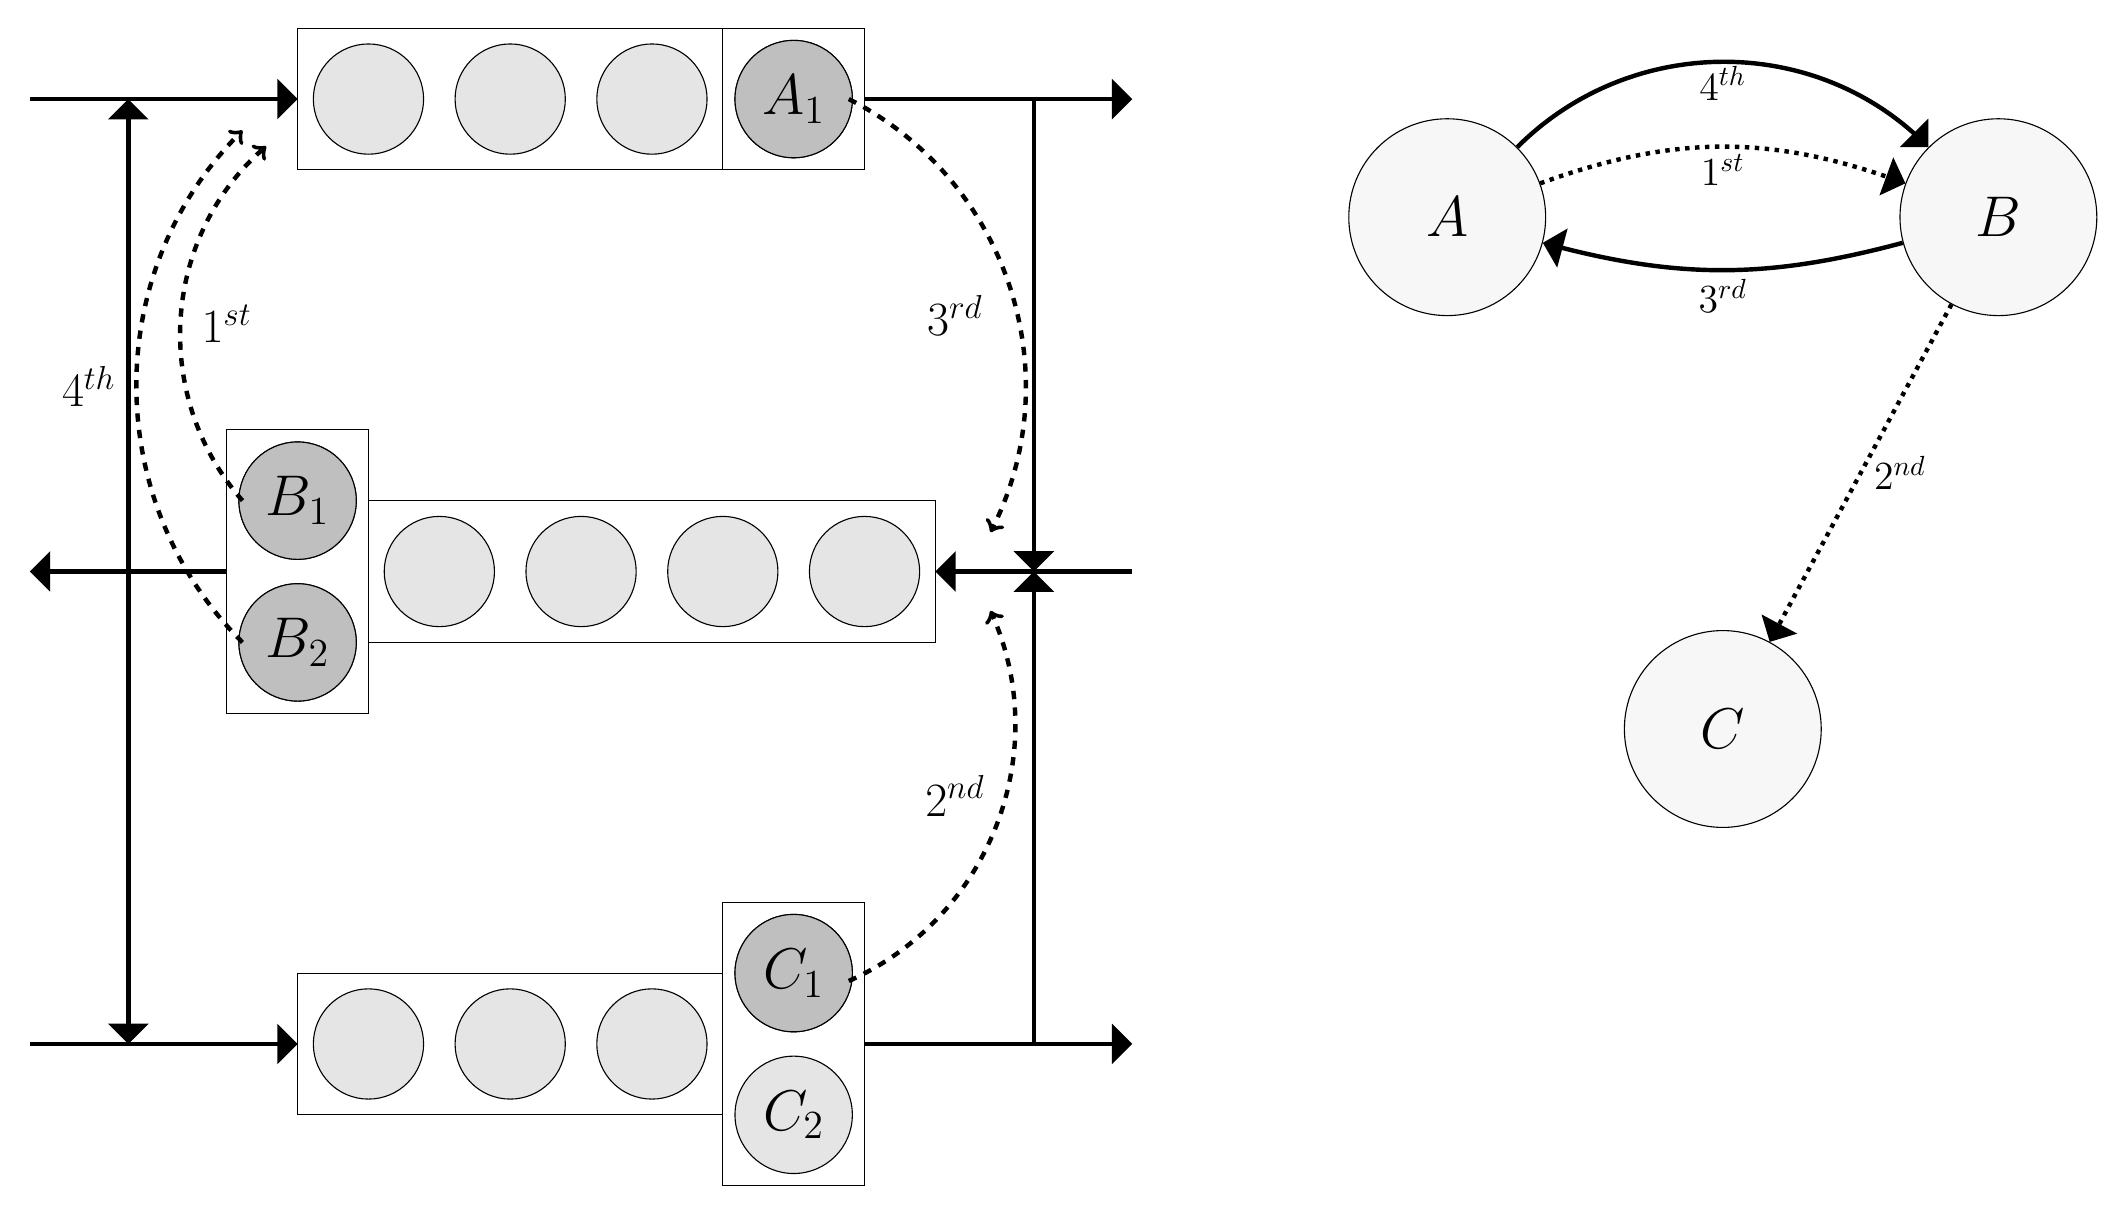
\begin{tikzpicture}

% Node bottom
\draw (3.9, 2.1) rectangle (9.3, 3.9);
\draw (9.3, 1.2) rectangle (11.1, 4.8);

% Node middle
\draw (4.8, 8.1) rectangle (12, 9.9);
\draw (3, 7.2) rectangle (4.8, 10.8);

% Node top
\draw (3.9, 14.1) rectangle (9.3, 15.9);
\draw (9.3, 14.1) rectangle (11.1, 15.9);

% Routings
\draw[ultra thick, -triangle 90] (0.5, 15) -- (3.9, 15); % In to top
\draw[ultra thick, -triangle 90] (11.1, 15) -- (14.5, 15); % Out of top

\draw[ultra thick, -triangle 90] (14.5, 9) -- (12, 9); % In to top
\draw[ultra thick, -triangle 90] (3, 9) -- (0.5, 9); % Out of top

\draw[ultra thick, -triangle 90] (0.5, 3) -- (3.9, 3); % In to bottom
\draw[ultra thick, -triangle 90] (11.1, 3) -- (14.5, 3); % Out of bottom

\draw[ultra thick, -triangle 90] (1.75, 9) -- (1.75, 15); % middle to top
\draw[ultra thick, -triangle 90] (1.75, 9) -- (1.75, 3); % middle to bottom

\draw[ultra thick, -triangle 90] (13.25, 15) -- (13.25, 9); % top to middle
\draw[ultra thick, -triangle 90] (13.25, 3) -- (13.25, 9); % bottom to middle

% Top customers
\node[align=center] [style={minimum size=1.4cm, text width=1.0cm, draw=black,fill=black!10,text=black,shape=circle}] at (10.2, 15) {\huge $A_1$};
\node[align=center] [style={minimum size=1.4cm, text width=1.0cm, draw=black,fill=black!10,text=black,shape=circle}] at (4.8, 15) {};
\node[align=center] [style={minimum size=1.4cm, text width=1.0cm, draw=black,fill=black!10,text=black,shape=circle}] at (6.6, 15) {};
\node[align=center] [style={minimum size=1.4cm, text width=1.0cm, draw=black,fill=black!10,text=black,shape=circle}] at (8.4, 15) {};

% Bottom customers
\node[align=center] [style={minimum size=1.4cm, text width=1.0cm, draw=black,fill=black!10,text=black,shape=circle}] at (3.9, 9.9) {\huge $B_1$};
\node[align=center] [style={minimum size=1.4cm, text width=1.0cm, draw=black,fill=black!10,text=black,shape=circle}] at (3.9, 8.1) {\huge $B_2$};
\node[align=center] [style={minimum size=1.4cm, text width=1.0cm, draw=black,fill=black!10,text=black,shape=circle}] at (5.7, 9) {};
\node[align=center] [style={minimum size=1.4cm, text width=1.0cm, draw=black,fill=black!10,text=black,shape=circle}] at (7.5, 9) {};
\node[align=center] [style={minimum size=1.4cm, text width=1.0cm, draw=black,fill=black!10,text=black,shape=circle}] at (9.3, 9) {};
\node[align=center] [style={minimum size=1.4cm, text width=1.0cm, draw=black,fill=black!10,text=black,shape=circle}] at (11.1, 9) {};

% Bottom customers
\node[align=center] [style={minimum size=1.4cm, text width=1.0cm, draw=black,fill=black!10,text=black,shape=circle}] at (10.2, 3.9) {\huge $C_1$};
\node[align=center] [style={minimum size=1.4cm, text width=1.0cm, draw=black,fill=black!10,text=black,shape=circle}] at (10.2, 2.1) {\huge $C_2$};
\node[align=center] [style={minimum size=1.4cm, text width=1.0cm, draw=black,fill=black!10,text=black,shape=circle}] at (4.8, 3) {};
\node[align=center] [style={minimum size=1.4cm, text width=1.0cm, draw=black,fill=black!10,text=black,shape=circle}] at (6.6, 3) {};
\node[align=center] [style={minimum size=1.4cm, text width=1.0cm, draw=black,fill=black!10,text=black,shape=circle}] at (8.4, 3) {};

% Alt State digraph Nodes
\node (A) [style={minimum size=2.5cm,draw=black,fill=black!3,text=black,shape=circle}] at (18.5, 13.5) {\huge{$A$}};
\node (B) [style={minimum size=2.5cm,draw=black,fill=black!3,text=black,shape=circle}] at (25.5, 13.5) {\huge{$B$}};
\node (C) [style={minimum size=2.5cm,draw=black,fill=black!3,text=black,shape=circle}] at (22, 7) {\huge{$C$}};

% B1 to A
\node[align=center] [style={minimum size=1.4cm, text width=1.0cm, draw=black,fill=black!25,text=black,shape=circle}] at (3.9, 9.9) {\huge $B_1$};
\node at (3, 12.15) {\LARGE $1^{st}$};
\draw[ultra thick, dotted, -triangle 90] (A) [bend left=20] to (B);
\draw[ultra thick, black, dashed, ->] (3.2, 9.9) [bend left=45] to (3.5, 14.4);
\node at (22, 14.1) {\Large $1^{st}$};

% B2 to A
\node[align=center] [style={minimum size=1.4cm, text width=1.0cm, draw=black,fill=black!25,text=black,shape=circle}] at (3.9, 8.1) {\huge $B_2$};
\node at (1.25, 11.35) {\LARGE $4^{th}$};
\draw[ultra thick, -triangle 90] (A) [out=45, in=135] to (B);
\draw[ultra thick, black, dashed, ->] (3.2, 8.1) [bend left=45] to (3.2, 14.6);
\node at (22, 15.2) {\Large $4^{th}$};


% C1 to B
\node[align=center] [style={minimum size=1.4cm, text width=1.0cm, draw=black,fill=black!25,text=black,shape=circle}] at (10.2, 3.9) {\huge $C_1$};
\node at (12.25, 6.15) {\LARGE $2^{nd}$};
\draw[ultra thick, dotted, -triangle 90] (B) -- (C);
\draw[ultra thick, black, dashed, ->] (10.9, 3.8) [bend right=45] to (12.7, 8.5);
\node at (24.25, 10.25) {\Large $2^{nd}$};

% A1 to B
\node[align=center] [style={minimum size=1.4cm, text width=1.0cm, draw=black,fill=black!25,text=black,shape=circle}] at (10.2, 15) {\huge $A_1$};
\node at (12.25, 12.25) {\LARGE $3^{rd}$};
\draw[ultra thick, -triangle 90] (B) [bend left=15] to (A);
\draw[ultra thick, black, dashed, ->] (10.9, 15) [bend left=45] to (12.7, 9.5);
\node at (22, 12.5) {\Large $3^{rd}$};

\end{tikzpicture}

\end{document}